\subsection{Block Fetching as a Bottleneck}~\label{ch3:sec:bfn}

\begin{figure}[h]
    \centering
    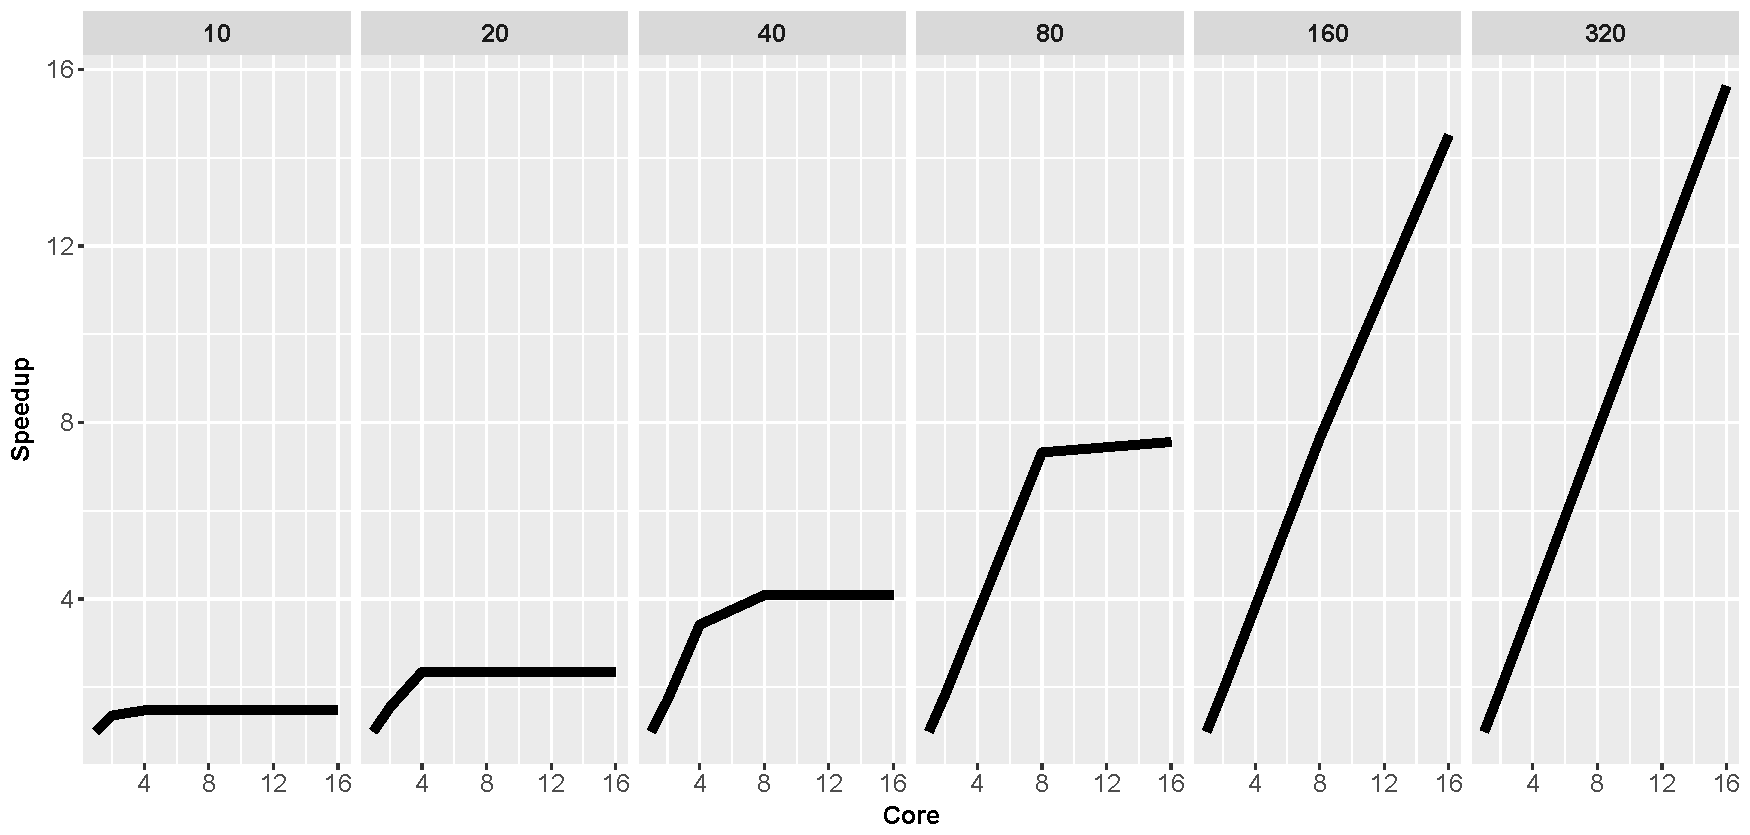
\includegraphics[width=1\textwidth]{chapter3/graphics/motivation_standard_fetch.pdf}

    \caption{Speedup of the synthetic benchmark when modifying the cycle length of the block (facets), over number of cores fused on the X axis. Higher is better.}
    \label{fig:block_graph}
\end{figure}

In a core-composition, the fetching mechanism operates in a round-robin fashion.
The first core in the composition starts by fetching blocks until all its lanes are full.
Once this happens, the first core then submits a block prediction to the next core in the composition.
The next core then operates in the same fashion, filling the lanes and then submitting another prediction to the next core in the composition.
After this prediction to the other core has been sent, the submitting core will no longer attempt any more fetches until another core sends it a new prediction.

With a round robin model can result in cores stalling due to having no blocks to execute.
This is due to the fact that a core can potentially commit all the blocks it has fetched and has not yet received a prediction from the previous core.
In that situation it has to wait for a signal from another core before continuing to fetch new blocks.
This means that cores in a composition are likely to stall when blocks are small.

Another concern with small, and especially quick to execute blocks is that cores in a composition may potentially never be utilised.
This comes from the fact that a core can only submit a prediction to the next core if all its lanes are full.
As a block can finish executing before a core has filled its lanes, this means that cores can potentially never submit a prediction to another core.

To understand how performance is affected by the block fetching mechanism, a synthetic benchmark which consists of a self-looping block was generated.
In this synthetic benchmark, an instruction is marked to have a variable cycle count which is defined ahead of time.
Using this variable cycle count, this allows to test how long -in terms of cycles- a block has to be before a core-composition becomes useful.
Figure~\ref{fig:block_graph} shows how core composition improves the performance of the synthetic benchmark when changing the number of cores being fused and the cycle length of the synthetic block.
The X axis plots the number of cores being fused, the Y axis represents the speedup which is measured by comparing the performance of a core composition to the performance of a single core.
Finally each facet represents the length of the synthetic block in cycles.

Figure~\ref{fig:block_graph} shows how, for core-compositions of sizes 4 and above require "long" blocks before becoming useful.
This is due to the fact that the time taken to populate all cores for large core-compositions takes longer than executing the blocks.
It is important to note that each core can fetch four of the synthetic blocks, meaning that a 16 core-composition would be fetching 64 blocks in total.
As it takes at least 2 cycles to make a prediction for the next block, it would take 128 cycles to populate all cores.
This explains why a 16 core-composition would require blocks to be at least of length 160 cycles before perceiving any performance benefits.

As single-lane blocks can be at most 32 instructions, and cores can execute up to two instructions per cycle, finding blocks that will satisfy such cycle requirements is difficult.
Thus, the block-fetching scheme can be considered a bottleneck in such cases.

\subsection{Inter-block communication}

In Chapter 2, the concept of inter-block memory dependencies was briefly mentioned as a potential issue for core-fusion.
This section covers how memory dependencies both in load/store instructions and register writes affect the performance on core-composition.
To understand how memory dependencies influence performance it is important to recall how EDGE handles memory instructions.
As previously stated in the EDGE instruction set architecture (ISA), architectural registers are only used for inter-block communication.
One of the main constraints of EDGE is that only non-speculative blocks can execute store instructions~\cite{smith2006compilingedge}.
This restriction is also applied to writes to registers.
When a speculative block attempts to execute a register read instruction, if an older block has a write to the same register that hasn't executed, the younger block must wait until the write has been executed.
Loads can be executed speculatively via store-set dependency predictor~\cite{chrysos1998storesets, smith2006compilingedge} to speed-up execution.
In case of memory violation from a speculative blocks, all blocks younger than the violating block and including the violating block must be flushed.

